% Created 2018-06-21 Thu 12:30
\documentclass[8pt]{beamer}
\usetheme{Montpellier}
\usecolortheme{dove}

\usepackage[sc,osf]{mathpazo}   % With old-style figures and real smallcaps.
\linespread{1.025}              % Palatino leads a little more leading
% Euler for math and numbers
\usepackage[euler-digits,small]{eulervm}
%\documentclass[10pt]{llncs}
%\usepackage{llncsdoc}
\usepackage{minted}
\usepackage[utf8]{inputenc}
\usepackage[T1]{fontenc}
\usepackage{fixltx2e}
\usepackage{graphicx}
\usepackage{longtable}
\usepackage{float}
\usepackage{wrapfig}
\usepackage{rotating}
\usepackage[normalem]{ulem}
\usepackage{amsmath}
\usepackage{textcomp}
\usepackage{marvosym}
\usepackage{wasysym}
\usepackage{amssymb}
\usepackage{hyperref}
\usepackage{polynom}
\renewcommand{\mod}[1]{\left( \texttt{mod}~#1 \right)}
\newcommand{\N}{\mathbb N}
\newcommand{\Z}{\mathbb Z}
\newcommand{\Q}{\mathbb Q}
\newcommand{\C}{\mathbb C}
\newcommand{\degree}{\texttt{degree}}
\tolerance=1000
\usetheme{Antibes}
\author{Siddharth Bhat}
\date{October 10th, 2019}
\institute{IIIT Theory group \\ Seminar Saturday}
\title{An introduction to the $p$-adics}
\hypersetup{
  pdfkeywords={},
  pdfsubject={},
  pdfcreator={Emacs 24.5.1 (Org mode 8.2.10)}}
\begin{document}

\maketitle

\begin{frame}[label=sec-1]{Why p-adics?}
Analogy between:
\begin{itemize}
\item $\mathbb Z$, \pause where $3, 5, 7, \dots$ are the ``primes''\pause
\item $\C[X]$, \pause where $(x - a)$ are the ``primes''\pause
\item $\C[X]$ has evaluation, taylor series. Can we access that in $\Z$?
\end{itemize}
\end{frame}

\begin{frame}{What is factorization?}

Remainder when factoring $p(x) = x^3 + x^2 + x + 1$ by $q(x) = x - 1$? \pause
\polylongdiv{X^3+X^2+X+1}{X-1}
\pause
$$(x^3+ x^2 + x + 1) = (x-1)(x^2 + 2x + 3) + 4$$
\pause
\begin{itemize}
\item $p(1) = 1^3 + 1^2 + 1 + 1 = 4$. Coincidence? \pause
\item Factoring out $q(x) = (x-1)$ \pause $ \simeq $ setting $q(x) = 0$ \pause : remove $q(x)$. \pause
\item setting $x - 1 = 0$, or setting $x = 1$ \pause
\item Substituting $x = 1$:  $p(1) = 1^3 + 1^2 + 1 + 1 = 4$ \pause
\end{itemize}

$$
\text{remainder of $p(x)$ on factoring $(x - a)$} \simeq \text{evaluation of $p(x_0)$ at $x_0 = a$}
$$
\end{frame}

\begin{frame}{What is evaluation in $\Z$?}

$$\text{remainder of $p(x)$ on factoring $(x - a)$} \simeq \text{evaluation of $p(x_0)$ at $x_0 = a$}$$
\pause
$$\text{evaluation of $p(x_0)$ at $x_0 = a$} \simeq \text{remainder of $p(x)$ on factoring $(x - a)$} $$
\pause
\begin{itemize}
\item $10(2)$ \pause $ = $ remainder of $10$ when factored by $2$; \pause $10 = 2\cdot5 + 0$\pause; $10(2) = 0$ \pause
\item $10(3)$ \pause $ = $ remainder of $10$ when factored by $3$; \pause $10 = 3\cdot3 + 1$ \pause; $10(3) = 1$ \pause
\item $10(5)$ \pause $ = $ remainder of $10$ when factored by $5$; \pause $10 = 5\cdot 2 + 0$ \pause; $10(5) = 0$ \pause
\item $10(7)$ \pause $ = $ remainder of $10$ when factored by $7$; \pause $10 = 7\cdot1 + 3$ \pause; $10(7) = 3$ \pause
\end{itemize}
\pause

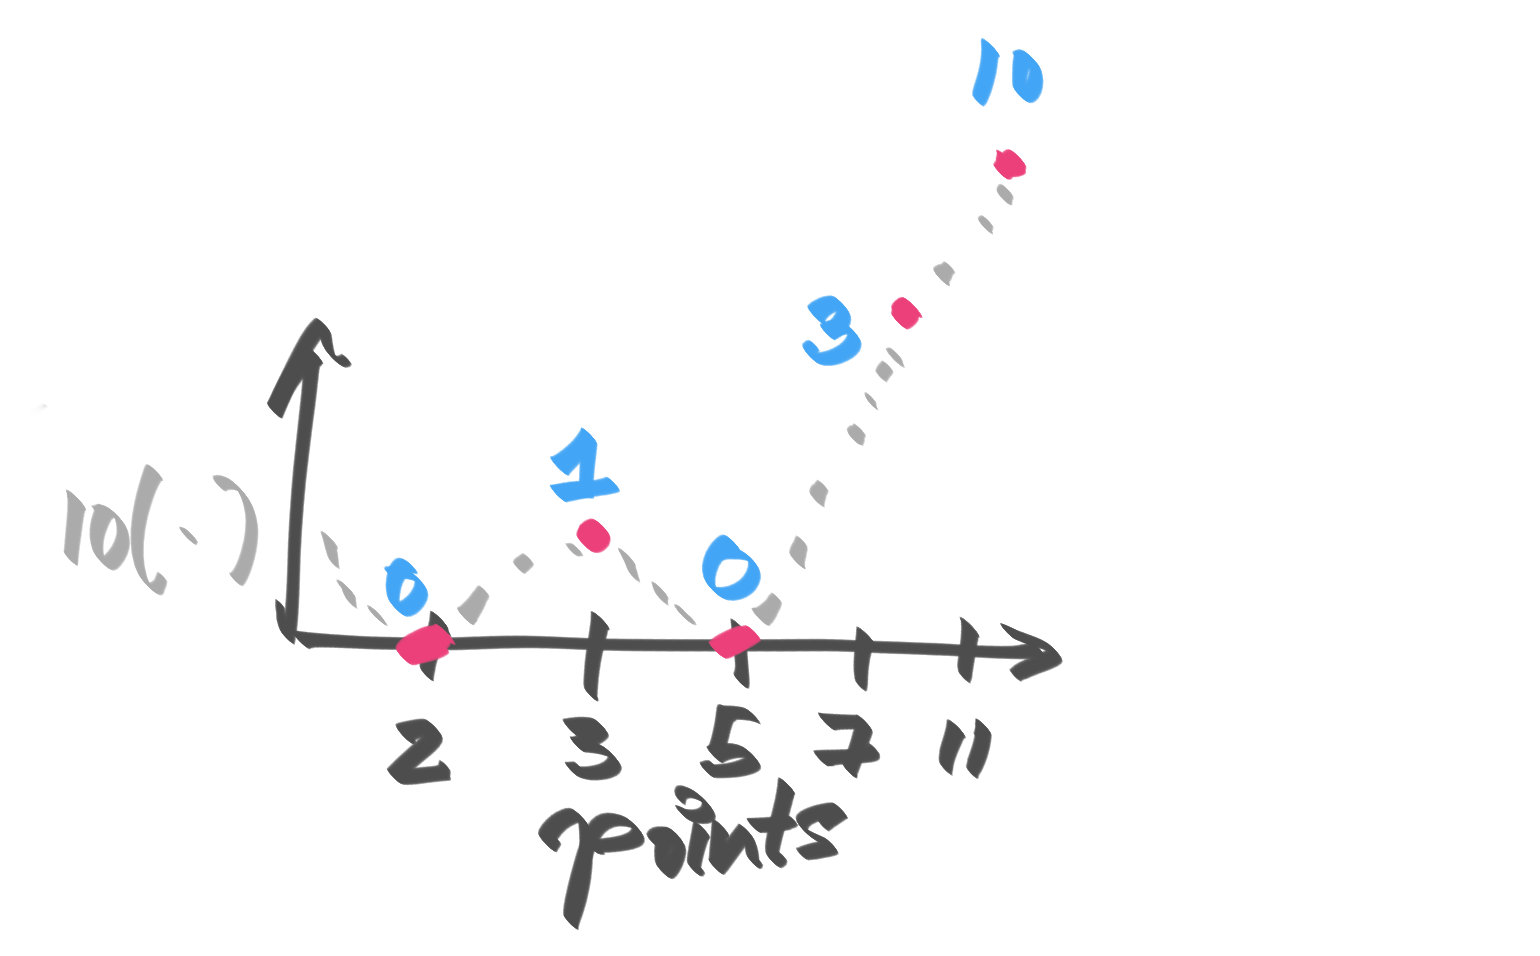
\includegraphics[width=3cm, height=3cm]{./10-as-a-fn.png}

\end{frame}

\begin{frame}{Why $n(p)$: only primes?}
\begin{itemize}
\item $10(5) = $ remainder of $10$ when factored by $5$; $10 = 5\cdot 2 + 0$ ; $10(5) = 0$
\item $10(7) = $ remainder of $10$ when factored by $7$; $10 = 7\cdot1 + 3$  ; $10(7) = 3$
\end{itemize}
\begin{itemize}
\item $p(x) = (x^2 - 15x + 50)$. \pause
\item $p(5) = $ \pause remainder of $p(x)$ when factored by $(x - 5)$; \pause 
\item $p(x) = (x-5)(x-10) + 0$; \pause $p(5) = 0$ \pause
\item $p(1) = $ \pause remainder of $p(x)$ when factored by $(x - 1)$; \pause 
\item $p(x) = (x-1)(x - 14) + 36$; \pause $p(1) = 36$ \pause
\end{itemize}

\pause

\begin{theorem}[Fundamental theorem of algebra] 
Every nonconstant polynomial $p(x) \in \C[X]$ can be written uniquely (upto reordering) as
a product of monic irreducibles of the form $(x - z_i)$ for $z_i \in C[X]$.
$$p(x) = \pm 1 \prod_i (x - z_i)$$
\end{theorem}

\pause

\begin{theorem}[Fundamental theorem of arithmetic] 
Every non-zero integer can be written uniquely (upto reordering) as a product of primes
$$n = \pm 1 \prod_i p_i$$
\end{theorem}

\end{frame}

\begin{frame}[fragile]{Cheap trick?}

\begin{itemize}
\item What are the complex numbers? \pause
\item $\mathbb R$ with $i$: $i^2 = -1$. \pause That is, $i^2 + 1 = 0$. \pause
\item Equivalently: $\mathbb R[X]$ \pause factored by by $q(x) = x^2 + 1$. \pause
\item Left with only linear polynomials. \pause
\item All higher power polynomials $h(x)$  are $h(x) = p(x) \cdot q(x) + r(x)$ \pause $\degree(r) \leq 1$. \pause
\item Example: $7x^2 + 5 = 7(x^2 + 1) - 2$ \pause
\item Sum of linear polynomials: $(a + xb) + (c + xd) = (a + c) + x(b + d) $\pause
\item Product of linear polynomials: $(a + xb) \cdot (c + xd) = ac + x(ad + bc) + bdx^2$ \pause
\item factoring product by $q(x) = x^2 + 1$:
\end{itemize}

\polylongdiv{bd x^2 + (ad + bc) x + ac }{x^2+1} \pause

\begin{block}{This is what we expect: Complex multiplication}
$(a + bi) (c + di) = (ad + bc) i + (ac - bd)$
\end{block}
\end{frame}

\begin{frame}{Taylor series}

\begin{itemize}
\item Taylor series of $q(x) \in \C[X]$ at $x = x_0$: $q(x) = \sum_i a_i (x - x_0)^i$ \pause
\item Taylor series of $n \in \Z$ at $p$ prime: $n = \sum_i b_i p^i$. \pause
\end{itemize}
\begin{definition}
The $p$-adic expansion of a natural number $n$ is
the unique decomposition $n = \sum_i b_i p^i$ for $0 \leq b_i < p$.
\end{definition}

\begin{itemize}
\item Taylor series of $q(x) = x^3 - 7x^2 + 15x - 9$  \pause at $x = 3$: \pause $q(x) =  2(x - 3)^2 + (x - 3)^3$ \pause
\item $q(x) = (x-3)^2(2 + (x-3))$ \pause $ = (x-3)^2(x-1)$ \pause
\item $x^3 - 7x^2 + 15x - 9$ has a root at $3$ of order $2$ \pause

\item Taylor series/p-adic expansion of $72$ at $p = 3$: \pause $72 = 0 \cdot 3 + 2 \cdot 3^2 + 2 \cdot 3^3$ \pause
\item $72 = 3^2 * (2 + 2 \cdot 3) = 3^2 * 2^3$ \pause
\item $72$ has a root at $p=3$ of order $2$ \pause
\end{itemize}
\end{frame}

\begin{frame}{Extending to the negatives}

\begin{itemize}
\item Consider $-1$. \pause
\item Goal: write $-1 = a_0 3^0 + a_1 3^1 + a_2 3^2 + a_3 3^3 + \cdots$.
\item $-1 \equiv -1 + 3 - 3$. \pause
\item $-1 \equiv 2 - 3$ \pause
\item $-1 \equiv 2 - 3 + 9 - 9$ \pause
\item $-1 \equiv 2 + (9 - 3) - 9$ \pause
\item $-1 \equiv 2 + 6 - 9$ \pause
\item $-1 \equiv 2 + 6 - 9 + 27 - 27$ \pause
\item $-1 \equiv 2 + 6 + (27 - 9) - 125$ \pause
\item $-1 \equiv 2 + 6 + 100 - 125$ \pause
\item $-1 \equiv 2 \cdot 3^0 + 2 \cdot 3^1 + 2 \cdot 3^2 + \cdots$. \pause
\end{itemize}
\end{frame}

\begin{frame}[fragile]{Checking our math: $-1 + 1$}

\begin{itemize}
\item $-1 \equiv 2\cdot 3^0 + 2\cdot 3^1 + 2 \cdot 3^2 + 2 \cdot 3^3 + \cdots$. \pause
\item $-1 +1 = \mathbf{1 + 2\cdot 3^0} +   + 2\cdot 3^1 + 2 \cdot 3^2 + 2 \cdot 3^3 + \cdots$. \pause
\item $-1 +1 = \mathbf{1 \cdot 3^1 + 2\cdot 3^1} + 2 \cdot 3^2 + 2 \cdot 3^3 + \cdots$. \pause
\item $-1 +1 = \mathbf{1\cdot 3^2 + 2 \cdot 3^2} + 2 \cdot 3^3 + \cdots$. \pause
\item $-1 +1 = \mathbf{1\cdot 3^3 + 2 \cdot 3^3} + \cdots$. \pause
\item $-1 +1 = \cdots$ \pause
\item $-1 +1 = 0$.
\end{itemize}
\end{frame}
\begin{frame}[fragile]{Positional notation}

\begin{columns}% [T] % align columns
\begin{column}{.23\textwidth}
\begin{minted}{text}

...22222
...00001 + 
----------
...?????
----------
\end{minted}
\end{column}
%
\begin{column}{.23\textwidth}
\pause
\begin{minted}{text}
      1
...22222
...00001 + 
----------
       0
----------
\end{minted}
\end{column}
%
\begin{column}{.23\textwidth} 
\pause
\begin{minted}{text}
     1 
...22222
...00001 + 
----------
      00
----------
\end{minted}
\end{column}
%
\begin{column}{.23\textwidth} 
\pause
\begin{minted}{text}
      
...22222
...00001 + 
----------
...00000
----------
\end{minted}
\end{column}
\end{columns}
\pause

\begin{itemize}
\item What is $-1$ is $2$ - adically? \pause
\item $-1 = \dots 11111$. \pause
\item Same as $2$'s complement!
\end{itemize}
\end{frame}

\begin{frame}{Rationals}
\begin{itemize}
\item Evaluate $1/4$ in the $3$-adic system. \pause
\item $1/4$ \pause $ = 1/(1+3)$ \pause $ = 1 - 3 + 3^2 - 3^3 + 3^4 + \dots$\pause
\item What is $-3$? that's not allowed! \pause
\item $3^2 = 3 \cdot 3$ \pause
\item $1/4 = 1 \mathbf{- 3 + 3\cdot 3} - 3^3 + 3^4 + \cdots$ \pause
\item $1/4 = 1  + \mathbf{2\cdot 3} - 3^3 + 3^4 + \cdots$ \pause
\item $1/4 = 1  + 2\cdot 3 \mathbf{- 3^3 + 3^4} + \cdots$ \pause
\item $1/4 = 1  + 2\cdot 3 \mathbf{- 3^3 + 3\cdot 3^3} + \cdots$ \pause
\item $1/4 = 1  + 2\cdot 3 + 2\cdot 3^3 + \cdots$ \pause
\item $1/4 = 1  + 2\cdot 3 + 2\cdot 3^3 + 2\cdot 3^5 + 2\cdot 3^7 + \cdots$ \pause
\item Similar cleverness produces $1/p$ for any rational. \pause
\end{itemize}
\end{frame}

\begin{frame}{A step back}
\begin{columns}
\begin{column}{.48\textwidth}
\begin{itemize}
\item Let $x = a_0 + a_1 p + a_2 p^2 + \dots$ \pause
\item  $x  \equiv a_0 ~\mod{p}$ \pause
\item  $x \equiv a_0 + a_1 p~~\mod{p^2} $ \pause
\item  $x - a_0 \equiv a_1 p~~\mod{p^2} $ \pause
\item  $x \equiv a_0 + a_1 p + a_2 p^2~\mod{p^3}$ \pause
\item  $x - a_0 - a_1 p \equiv a_2 p^2~\mod{p^3}$ \pause
\end{itemize}
% \noindent\rule{2cm}{0.4pt}
% {\footnotesize
% \begin{itemize}
% \item $72 = a_0 + 3 a_1 + 9 a_2 + 27 a_3 + 81 a_4 \dots$\pause
% \item $72 \equiv a_0 ~\mod{3}$\pause; $a_0 \equiv 0~\mod{3}$\pause
% \item $72 \equiv 0 + 3 a_1~\mod{9}$\pause; $3a_1 \equiv 0~\mod{3}$\pause
% \item $72 \equiv 0 + + 0 9 a_1~\mod{27}$\pause; $9a_2 \equiv 17~\mod{27}$\pause
% \end{itemize}
% }
\end{column}

\begin{column}{.48\textwidth}
{\footnotesize
\begin{itemize}
\item Let $-1 = \sum_i a_i 3^i$ \pause
\item Let $-1 = a_0 ~\mod{3}$\pause; $a_0 = 2~\mod{3}$\pause
\item Let $-1 = 2  + a_1 \cdot 3~\mod{9}$; \pause $-3 = a_1 \cdot 3~\mod{9}$; \pause $6 = a_1 \cdot 3~\mod{9}$; \pause $a_1 = 2$
\item Let $-1 = 2 + 2 \cdot 3 + 2 \cdot 3^2 + \dots$
\end{itemize}
\noindent\rule{2cm}{0.4pt}
\begin{itemize}
\item Let $1/4 = \sum_i a_i 3^i$ \pause
\item What defines $1/4$? \pause The equation $1/4 \cdot 4 = 1$.\pause
\item $(a_0 + 3a_1 + 9a_2 + \dots)(1 + 3 + 0 \cdot 9 + \cdots) = 1$\pause
\item $a_0 \cdot 1 \equiv 1~\mod{3}$\pause $a_0 = 1$.\pause
\item $(1 + 3a_1) (1 + 3) \equiv 1~\mod{9}$\pause  $4 + 12 a_1 \equiv 1~\mod{9}$\pause
\item $3a_1 \equiv -3 \equiv 6~\mod{9}$ \pause
\item $a_1 \equiv 2\mod{9}$\pause
\item $1/4 = 1 + 2\cdot 3 + 2 \cdot 3^3 + \dots$
\end{itemize}
}
\end{column}
\end{columns}
\end{frame}

\begin{frame}{Irrationals}
\begin{itemize}
\item Let's solve $X^2 = 2$ in the $7-$adics. \pause
\item Such a solution does not "really exist" in the rationals or the integers.\pause
\item Let $x = \sum_i a_0 + 7 a_1 + 49 a_2 + \dots$\pause
\item Start with $x^2 \equiv a_0^2 \equiv 2 ~\mod{7}$\pause
\item $a_0 = 3$
\item $(3 + 7a_1)^2 \equiv 2 ~\mod{49}$\pause
\item $9 + 42a_1 + 49a_1^2 \equiv 2 ~\mod{49}$\pause
\item $7 + 42a_1  \equiv 0 ~\mod{49}$\pause
\item $-42 + 42a_1  \equiv 0 ~\mod{49}$\pause
\item $a_1  \equiv 1 ~\mod{49}$\pause
\item Keep going to extract $a_2, a_3, \dots$\pause
\item We solved an equation in $\Q_7$ for which we didn't have a solution in $\Q$!\pause
\item Can we always lift? \textbf{Hensel's lemma}
\end{itemize}
\end{frame}


\begin{frame}{Convergence}

\begin{itemize}
\item Intuition: higher powers of $p$ should become ``smaller'' for convergence! \pause
\item $|a|_p = p^{-1 \cdot \text{highest power of } p \text { which divides } a}$\pause
\item $|10|_3 = 3^{-0} = 1$\pause
\item $|3|_3 = 3^{-1} = 1/3$\pause
\item $|9|_3 = 3^{-2} = 1/9$\pause
\item $|90|_3 = 3^{-2} = 1/9$\pause
\item $|27|_3 = 3^{-3} = 1/27$\pause
\item $|ab|_p = |a|_p \cdot |b|_p$. Plays well with multiplication \pause
\item What about addition? \pause
\item $|a+b|_p \leq \max(|a|_p, |b|_p)$\pause
\item Let $a = p^\alpha a'$, $b = p^\beta b'$, let $\alpha \leq \beta$ WLOG.\pause
\item $(a + b) = p^\alpha (a' + p^{\beta - \alpha} b')$\pause
\item If $(a' + p^{\beta - \alpha} b')$ is \emph{not} divisible by $p$ \pause , then $|a+b|_p = p^{-\alpha} = |a|_p$\pause
\item If $(a' + p^{\beta - \alpha} b')$ \emph{is} divisible by $p$ \pause, then $|a+b|_p = p^{-(\alpha + \texttt{more})} < p^{-\alpha}$\pause
\item $|10|_2 = |2 * 5|_2 = 1/2$; $|40|_2 = |8 * 5|_2 = 1/8$\pause
\item $|10 + 40|_2 = |50|_2 = |2 * 25|_2 = 1/2$\pause
\item $|10 + 10|_2 = |20|_2 = |4 * 5|_2 = 1/4$\pause
\end{itemize}
\end{frame}

\begin{frame}{Scam v/s non-scam}
\begin{itemize}
\item Solve $x = 1 + 3x$\pause
\item \textbf{Non scam}:$-2x = 1$\pause; $x = -1/2$\pause
\item Recurrence: $x[i+1] = 1 + 3x[i]$\pause
\item $x_0 = 1$\pause
\item $x_1 = 1 + 3$
\item $x_2 = 1 + 3x_1 = 1 + 3(1 + 3) = 1 + 3 + 3^2$\pause
\item $x_3 = 1 + 3x_2 = 1 + 3(1 + 3 + 3^2) = 1 + 3 + 3^2 + 3^3$\pause
\item $x_i = 1 + 3 + 3^2 + \dots + 3^i$\pause
\item $x_\infty = 1/(1-3) = -1/2$
\item Converges? We need $|3| < 1$\pause
\item But it is! $|3|_3 < 1$\pause
\end{itemize}
\end{frame}

\begin{frame}[fragile]{Why only primes? Geometry of functions}
% \begin{itemize}
% \item Dividing $p(x)$ by $(x-a_0)$ $\simeq$ evaluating  $p(x)$ at $x = a_0$ \pause
% \item Dividing $z \in \mathbb Z$ by $a_0 \in \mathbb Z$ $\simeq$ evaluating $z$ at $a_0$? \pause
% \end{itemize}
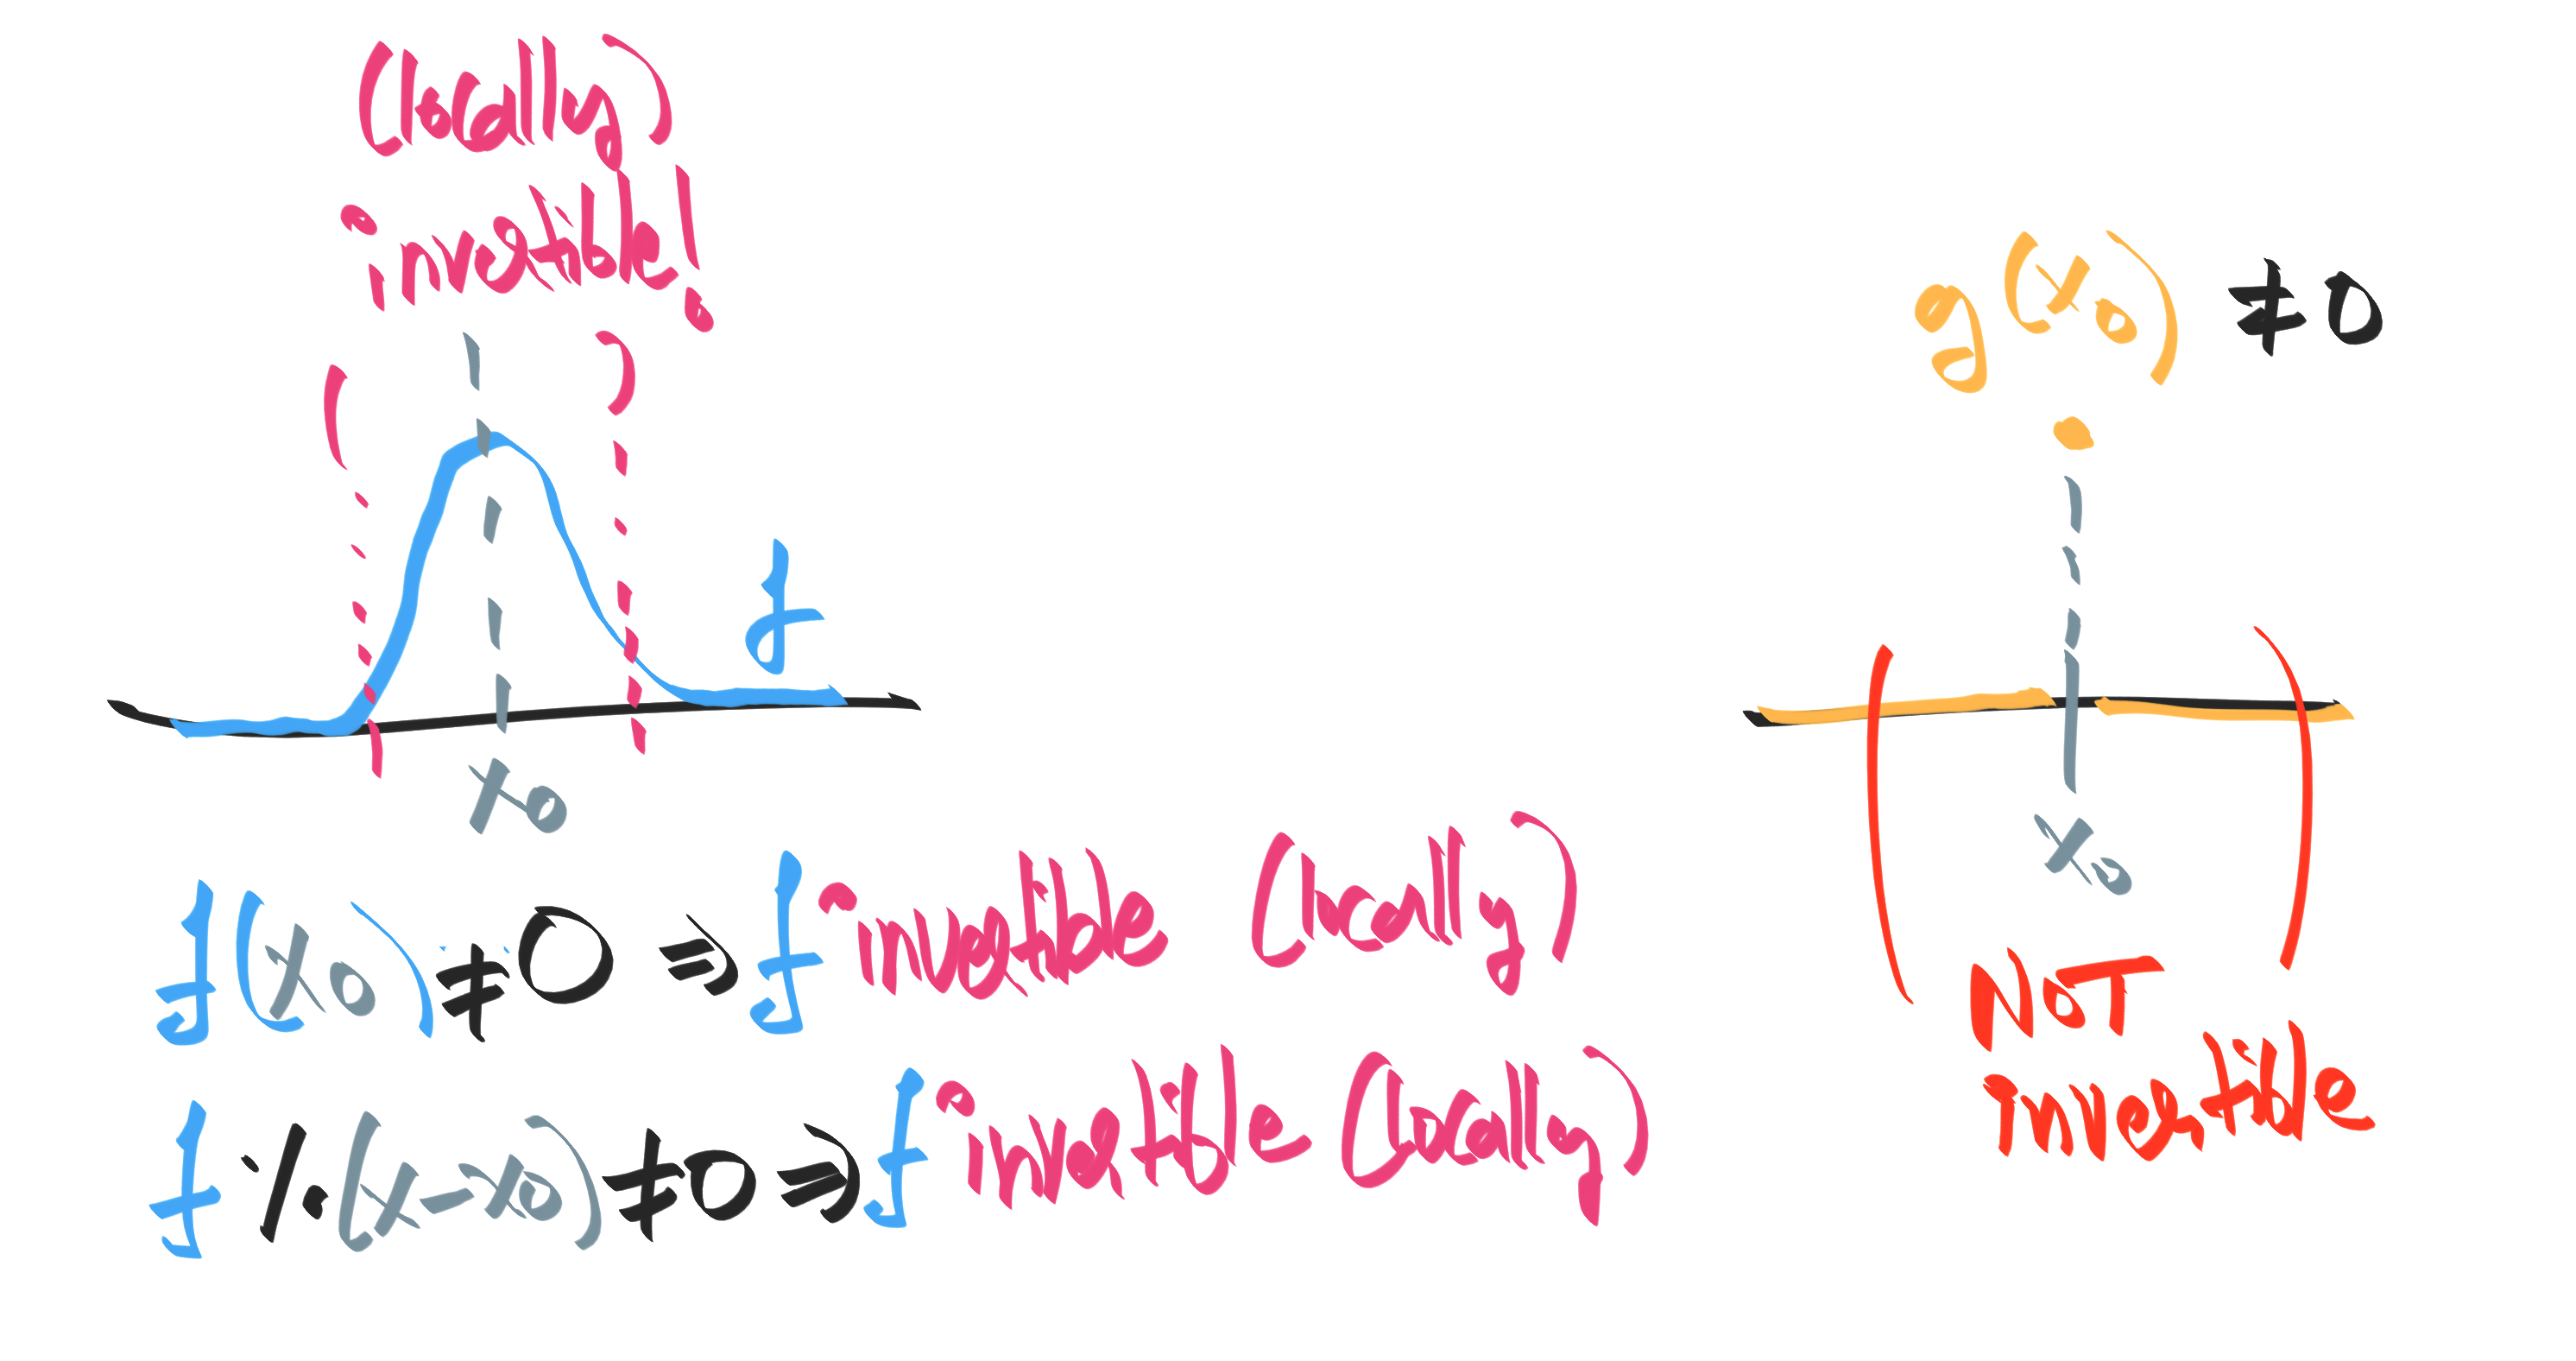
\includegraphics[height=5cm]{./nonzero-fn-locally-invertible.png}\pause
\begin{itemize}
\item $f(x)$: continuous, \emph{non-zero} at $x = x_0$. \pause
\item $f(x)$: \emph{locally invertible} at $x = x_0$. \pause
\end{itemize}
\end{frame}

\begin{frame}[fragile]{Why only primes? Geometry of numbers}

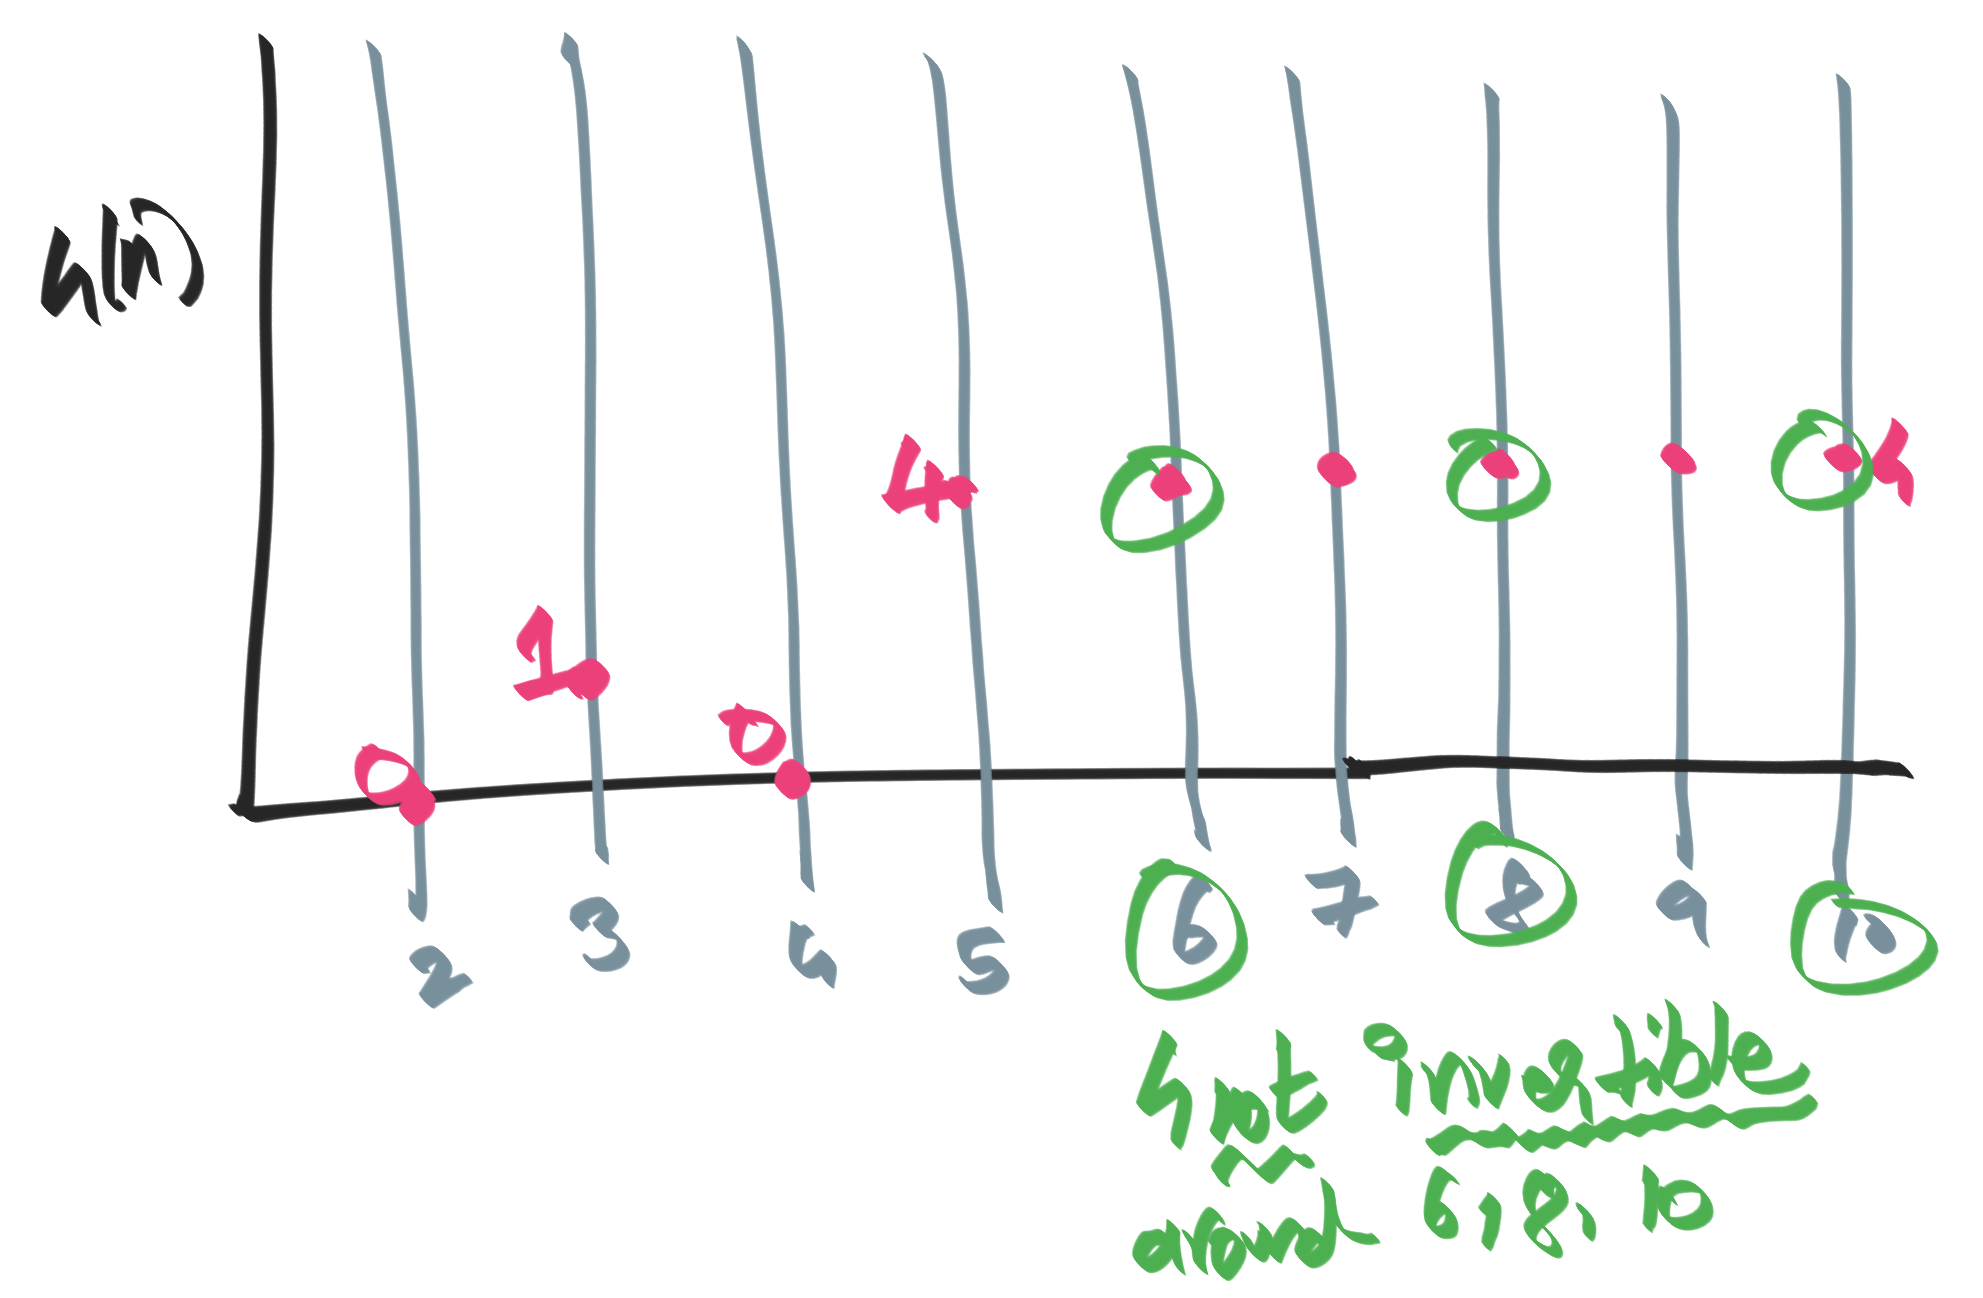
\includegraphics[height=4cm]{./fn-4-on-naturals.png}
\begin{itemize}
\item consider $4(\cdot)$ as function $\mathbb N \rightarrow \mathbb N$. \pause
\item nonzero at $a_0 = 6$: $4 \simeq 4~\mod{6}$\pause
\item \emph{not invertible} modulo $6$: $[0, 1, 2, 3, 4, 5] \times 4 \equiv [0, 4, 8, 12, 16, 20] \equiv [0, 4, 2, 0, 4, 2] \mod{6}$ \pause
\item If we want $4$ to be a \emph{continuous} function\pause
\item then 6 should not be a point!
\item The only points in $\N$ which obey ``any non zero function is locally invertible'' are primes.
\item Hence, we only consider evaluation at primes.
\end{itemize}
\end{frame}

\begin{frame}[fragile]{Why is this useful?}
\begin{itemize}
\item Does $x^2 = 2$ have a solution in $\mathbb Z$?
\item If it has a solution in $\mathbb Z$ \pause
\item It must continue to have solutions in $Z/n\Z$\pause
\item $a \cdot b = c \implies a \cdot_n b \equiv c ~\mod{n}$, $a + b = c \implies a +_n b \equiv c~\mod n$\pause
\item $x^2 = 2~\mod{5}$: $[0, 1, 2, 3, 4]^2 = [0, 1, 4, 9, 16] = [0, 1, 4, 4, 1]$
\item So $x^2 = 2$ has no solution in $\mathbb Z$
\item We used a \emph{finite number of candidates} in $\Z/5Z$ \pause, eliminated infinite number of candidates in $\Z$.
\item Hasse Minkowski: A quadratic form ($ax^2 + bxy + cy^2$) has a root in $\Q$ iff it has roots in all $\Q_p$.
\end{itemize}
\end{frame}

\begin{frame}{Hensel's Lemma}
\begin{theorem}
\begin{itemize}
\item Let $f(x)$ be a polynomial with integer or $p$-adic coefficients.
\item If $f(r) \equiv 0 ~\mod{p^k}$ and $f'(r) \not \equiv 0 ~\mod{p}$ [non-degenerate], then
\item (1) there is an integer $s$ such that $f(s) \equiv 0 ~\mod{p^{k+1}}$ [lifting]
\item (2) and $r \equiv s~\mod{p^k}$ [consistency]
\end{itemize}
\end{theorem}

{\footnotesize
\begin{itemize}
\item Since $r \equiv s~\mod{p^k}$ [consistency], we have $s =  r + tp^k$ for some $t \in \Z$.\pause
\item If we find a $t$, then we are done, since that is the unknown to find $s$. \pause
\item $f(s) = f(r + tp^k) = f(r) + f'(r) tp^k + (tp^k)^2(\dots)$.\pause
\item $f(s) = f(r + tp^k) = f(r) + f'(r) tp^k + p^{2k}t^2 g(t)$ for some $g(t) \in \Z[t]$.\pause
\item Since $f(r) \equiv 0~\mod{p^k}$, we have $f(r) = zp^k$ for some $z \in \Z$.\pause
\item $f(s) = f(r + tp^k) = zp^k + f'(r) tp^k +  p^{2k}t^2 g(t)$.\pause
\item $f(s) = f(r + tp^k) = p^k(z + f'(r) t) +  p^{2k}t^2 g(t)$.\pause
\item We need $f(s) \equiv 0 ~\mod{p^{k+1}}$  for [lifting].
\item $f(s) \equiv 0 ~\mod{p^{k+1}}$ iff $p^k(z + f'(r) t) \equiv 0 ~\mod{p^{k+1}}$ (Substituting $f(s)$, terms die: $p^{k+2}$ factor)\pause
\item $(z + f'(r)t) \equiv 0 \mod{p}$ [$p^k$ factors common]
\item $tf'(r) \equiv -z ~\mod{p}$. Hence, $t = z[f'(r)]^{-1}~ \mod{p}$.
\item $f'(r)$ will have an inverse  if $f'(r) \not \equiv 0 ~\mod{p}$ by virtue
      of being prime.
\end{itemize}
}
\end{frame}


\end{document}
